\subsection{Generación de la tensión de excitación}

Se emplea la referencia MCP1541 para proporcionar una excitación estable de \SI{4.096}{\V} al puente de Wheatstone, con una tolerancia de \(\pm\SI{0.1}{\percent}\) y un coeficiente de temperatura de \SI{50}{ppm\per\celsius} \cite{mcp6021_datasheet}. El circuito incorpora dos condensadores de desacoplo en el pin de salida para atenuar transitorios y ruido de alta frecuencia.

\begin{figure}[H]
    \centering
    \begin{subfigure}[b]{0.48\textwidth}
        \centering
        %\includesvg[width=\textwidth]{figs/CKTO VREF}
        \caption{Esquema del circuito.}
        \label{fig:vref_esquema}
    \end{subfigure}
    \hfill
    \begin{subfigure}[b]{0.48\textwidth}
        \centering
        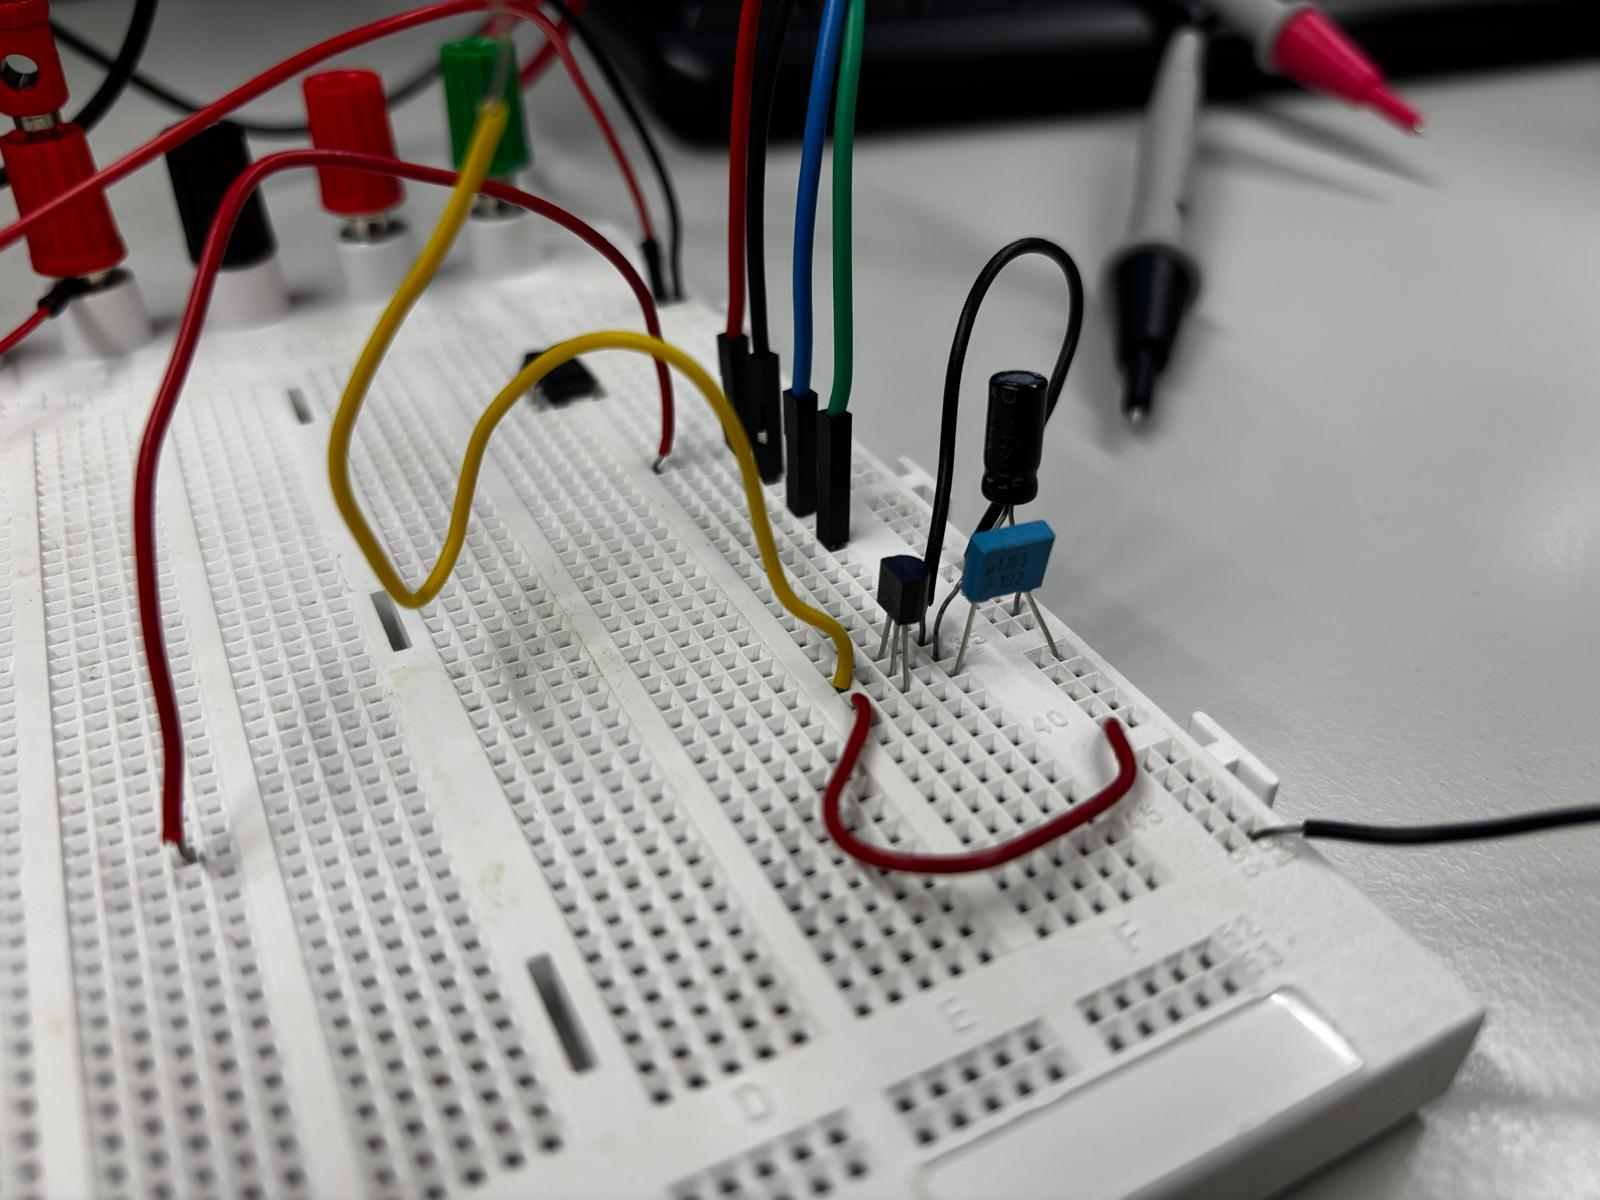
\includegraphics[width=\textwidth]{figs/vref_implementation.jpeg}
        \caption{Montaje en la \textit{protoboard}.}
        \label{fig:vref_impl}
    \end{subfigure}
    \caption{Circuito de generación de \texttt{VREF} mediante la referencia MCP1541.}
    \label{fig:vref}
\end{figure}

El valor medido experimentalmente es $V_{\mathrm{REF}} = \SI{4.1}{\V}$, lo que representa una desviación del \SI{0.097}{\percent} respecto al nominal \cite{microchip_mcp1525_2012}, dentro de la tolerancia especificada por el fabricante.

\subsection{Generación del pedestal de referencia}

Sin un nivel de referencia en el pin REF del AD623, cualquier desequilibrio de polaridad negativa en el puente empujaría la salida del amplificador hacia \SI{0}{\V}, provocando saturación. Para evitarlo, se inyecta un pedestal en el pin~5 (REF) del AD623 mediante un divisor resistivo aislado por un seguidor de tensión basado en el MCP6021 \cite{mcp6021_datasheet}.

\subsubsection*{Diseño inicial: $R_2 = \SI{22}{\kohm}$}

En una primera iteración, el divisor se dimensiona con $R_1 = \SI{68}{\kohm}$ y $R_2 = \SI{22}{\kohm}$, obteniendo un pedestal teórico de:

\[
    V_{\mathrm{PED,1}} = \SI{4.096}{\V} \cdot
    \frac{\SI{22}{\kohm}}{\SI{68}{\kohm} + \SI{22}{\kohm}}
    \approx \SI{1.0}{\V}
\]

El valor medido experimentalmente fue $V_{\mathrm{PED,1,med}} = \SI{0.9945}{\V}$, dentro de la
tolerancia esperada. Sin embargo, con este pedestal la tensión de salida del sistema con la botella de \SI{1}{\kg} resultó ser $V_{o,\mathrm{botella,1}} = \SI{2.20}{\V}$, lo que dejaba
un margen de excursión reducido hacia la plena escala (\SI{1.5}{\kg}) y comprometía la resolución efectiva del sistema.

\subsubsection*{Ajuste final: $R_2 = \SI{44}{\kohm}$}

Para aumentar la excursión de la señal de salida y mejorar la resolución, se añadió una resistencia adicional de \SI{22}{\kohm} en serie con $R_2$, elevando el pedestal a:

\[
    V_{\mathrm{PED,2}} = \SI{4.096}{\V} \cdot
    \frac{\SI{44}{\kohm}}{\SI{68}{\kohm} + \SI{44}{\kohm}}
    \approx \SI{1609.14}{\mV}
\]

Con este nuevo pedestal, la tensión de salida con la botella de \SI{1}{\kg} pasó a ser $V_{o,\mathrm{botella,2}} = \SI{2.819}{\V}$, lo que representa un incremento de \SI{0.619}{\V} respecto a la configuración anterior y amplía el rango dinámico aprovechable de la señal. El valor medido del pedestal fue $V_{\mathrm{PED,2,med}} = \SI{1.597}{\V}$, con una desviación de \SI{0.754}{\percent} respecto al valor teórico, atribuible a las tolerancias del 5\,\% de las resistencias.

Aunque el valor final del pedestal difiere del valor de \SI{1.0}{\V} nominal indicado en el enunciado, sigue cumpliendo el objetivo fundamental de mantener la salida del AD623 alejada de la saturación de masa en el peor escenario de desequilibrio del puente, garantizando además un mayor aprovechamiento del rango de entrada de la tarjeta DAQ.

\begin{figure}[H]
    \centering
    %\includesvg[width=0.65\textwidth]{figs/CKTO MCP6021}
    \caption{Circuito generador del pedestal de referencia
        en su configuración final: divisor resistivo
        ($R_1 = \SI{68}{\kohm}$,
        $R_2 = 2 \times \SI{22}{\kohm} = \SI{44}{\kohm}$)
        y seguidor MCP6021 con salida al pin~5 (REF)
        del AD623.}
    \label{fig:pedestal}
\end{figure}


\subsection{Análisis de Tolerancias (Worst-Case DC)}

En esta sección se presenta la tensión de error máxima prevista a la salida del sistema de acondicionamiento bajo condiciones de reposo (sin carga aplicada). Se implementó el modelo de análisis para el peor escenario, este modelo asume la superposición lineal de todas las fuentes de error del sensor y de la etapa de amplificación, alineadas en la polaridad más desfavorable para inducir la máxima desviación posible antes de la saturación del sistema.

\subsubsection{Cálculo del error inherente del sensor}

El primer término de error proviene del desequilibrio físico del puente de Wheatstone. Se estableció un desequilibrio sin carga equivalente al 5\% de la salida a fondo de escala (FSO). Considerando la tensión de excitación unipolar de 4.096 voltios (proporcionado por la referencia del MCP1541) y la sensibilidad nominal de la célula de carga de 1 $\text{mV/V}$, la salida a fondo de escala se define como:

$$V_{FSO}=V_{EXC} \cdot \text{Sensibilidad} = 4.096 \text{V} \cdot 1 \text{ mV/V} = 4.096 \text{ mV}$$

Por lo que la tensión de error diferencial intrínseca aportada por el sensor en reposo es:

$$V_{err\_sensor}=0.05 \cdot V_{FSO} = 0.05 \cdot 4.096 \text{ mV} = 0.2048 \text{ mV}$$

\subsubsection{Error de la etapa de amplificación}

La segunda etapa de error derivó del amplificador de instrumentación AD623. En el diseño implementado, la ganancia (G) se fijó mediante una resistencia $R_{G} = 50.2 \text{ }\Omega $. Aplicando la ecuación de la ganancia del fabricante \cite{ad623_datasheet}:

$$\text{GAIN} = 1+100\text{ k}\Omega/R_G = 1+100\text{ k}\Omega/50.2\text{ }\Omega$$
$$\text{GAIN} = 1993.032 \text{ V/V} $$

\subsubsection{Errores referidos a la entrada (amplificados por la ganancia G)}

\begin{itemize}
    \item Tensión de offset de entrada ($V_{OSI}$): De acuerdo con las especificaciones del fabricante \cite{ad623_datasheet}, el valor máximo es de 200 $\mu$ \unit{V} = 0.2 m\unit{V}
    \item Caída de tensión por la corriente de offset ($V_{err\_IB}$): En el esquema de diseño, las entradas del AD623 están precedidas por un filtro pasivo contra interferencias de radiofrecuencia (RFI) compuesto por las resistencias R1 = R2 = 15.9 k $\Omega$. Al circilar la corriente de offset de entrada ($I_{OS}$) (de acuerdo con \cite{ad623_datasheet}, es de 2 \text{ nA}), a través de estas resistencias, se induce un error diferencial adicional evaluado en:
          $$V_{err\_IB} = I_{OS} \cdot R_{filtro} = 2 \text{ nA} \cdot 15.9 \text{ k} \Omega=  0.0318 \text{ mV}$$
\end{itemize}

\subsubsection{Errores referidos a la salida (independientes de la ganancia)}

\begin{itemize}
    \item Tensión de offset de salida ($V_{OSO}$): El fabricante especifica un valor máximo de 1000 $\mu$V = 1 m\unit{V}.
\end{itemize}

\subsubsection{Ecuación global del peor escenario y contraste de saturación}

Aplicando el factor de amplificación de la etapa (G = 1993.032 V/V), solo a las perturbaciones generadas a la entrada del sistema, la ecuación analítica del error máximo en corriente continua es:

$$V_{error\_MAX}=G \cdot (V_{err\_sensor} + V_{OSI} + V_{err\_IB}) + V_{OSO}$$

$$V_{error\_MAX}= 1993.032 \cdot (0.2048 \text{ mV} + 0.2 \text{ mV} + 0.0318 \text{ mV}) + 1 \text
    { mV}$$

$$V_{error\_MAX}= 871.16 \text
    { mV}$$

Para determinar la tensión estática absoluta en el terminal de salida del acondicionador ($V_{OUT\_reposo}$), se debe superponer el voltaje del pedestal virtual de 1609.14 m\unit{V}, introducido en el terminal de referencia (REF) del AD623 mediante la etapa aislada del amplificador operacional MCP6021.

$$ V_{OUT\_reposo} = V_{pedestal} \pm V_{error\_MAX} = 1609.14 \text{ mV} \pm 871.16 \text{ mV} $$

$$ V_{OUT\_reposo} = \{737.98 \text{ - } 2480.3\} \text{ mV}$$

De acuerdo con el resultado anterior, se puede constatar que el nivel de tensión en reposo se mantiene dentro del rango de trabajo de la entrada analógica de la tarjeta DAQ NI USB-6001.